\scanpage{20}
\begin{center}--- 48 ---\end{center}
\margin{\figure{\begin{tikzpicture}\draw (0,0)--(.01,.45);\end{tikzpicture}}}

1) Le groupe $\mathrm G_{\mathrm V}$ est un sous-groupe \textit{ouvert} du groupe $\mathrm H_{\mathrm V}(\mathbf Q_p)$ des points de $\mathrm H_{\mathrm V}$ à coefficients dans $\mathbf Q_p$.

Il revient au même de dire que l'algèbre de Lie du groupe analytique $p$-adique $\mathrm G_{\mathrm V}$ est \textit{algébrique}, au sens de Chevalley.

2) La décomposition $\mathrm V_{\mathrm C}=\sum\mathrm V_{\mathrm C}(n)$ définit un homomorphisme
\[
h:\mathbf G_m/_{\mathrm C}\to\mathbf{GL}_{\mathrm V}/_{\mathrm C}
\]
de groupes algébriques sur $\mathrm C$. Soit $\mathrm H_{\mathrm V}^{\unsure{0|\circ}}$ la composante neutre de $\mathrm H_{\mathrm V}$, et soit $\mathrm H_{\mathrm V}^{\unsure{0|\circ}}/_{\mathrm C}$ le sous-groupe de $\mathbf{GL}_{\mathrm V}/_{\mathrm C}$ déduit de $\mathrm H_{\mathrm V}^{\unsure{0|\circ}}$ par extension des scalaires de $\mathbf Q_p$ à $\mathrm C$. Alors \textit{$\mathrm H_{\mathrm V}^{\unsure{0|\circ}}/_{\mathrm C}$ contient le groupe $h(\mathbf G_m/_{\mathrm C})$}, image de $h$.

Lorsque de plus $\mathrm G_{\mathrm V}$ est \textit{résoluble}, on peut caractériser $\mathrm H_{\mathrm V}^{\unsure{0|\circ}}$ comme \textit{le plus petit sous-groupe algébrique} $\mathrm R$ sur $\mathbf Q_p$ de $\mathbf{GL}_{\mathrm V}$ \textit{tel que $\mathrm R/_{\mathrm C}$ contienne $h(\mathbf G_m/_{\mathrm C})$}; c'est l'analogue $p$-adique du \textit{groupe de Mumford-Tate}.

Il est probable que cette caractérisation de $\mathrm H_{\mathrm V}^{\unsure{0|\circ}}$ vaut sans supposer $\mathrm G_{\mathrm V}$ résoluble; on pourrait le prouver si l'on savait que $\mathrm V_{\mathrm C}=\mathrm V_{\mathrm C}(0)$ entraîne que $\mathrm G_{\mathrm V}$ est fini.
\margin{\figure{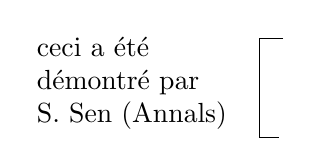
\begin{tikzpicture}[x=1cm,y=1cm]
\node[anchor=north west,align=left] at (0,1.4) {ceci a été\\démontré par\\S. Sen (Annals)};
\draw (3.25,1.25)--(2.95,1.25)--(2.95,0)--(3.2,0);
\end{tikzpicture}}}

3) Lorsque $\mathrm V$ varie, les groupes $\mathrm H_{\mathrm V}$ forment un système projectif; leur limite projective est un \textit{groupe proalgébrique} $\mathrm H$ sur $\mathbf Q_p$, muni d'un homomorphisme $h:\mathbf G_m/_{\mathrm C}\to\mathrm H/_{\mathrm C}$. La catégorie des modules de Hodge est équivalente à celle des $\mathrm H$-modules de dimension finie; si $\mathrm H^{\unsure{0|\circ}}$ désigne la composante neutre de $\mathrm H$, le groupe $\mathrm H/\mathrm H^{\unsure{0|\circ}}$ est le groupe de dimension zéro associé au groupe profini $\mathrm G$; le groupe $\mathrm H^{\unsure{0|\circ}}$ ne change pas lorsqu'on remplace $\mathrm K$ par une extension finie.

4) Soit $\Theta$ le plus grand quotient commutatif du groupe proalgébrique $\mathrm H^{\unsure{0|\circ}}$. Le groupe $\Theta$ est une limite projective de tores; il ne dépend que de $p$ (mais pas de $\mathrm K$); on a:
\[
\Theta=\underset{\leftarrow}{\lim.}\,\mathrm T_{\mathrm E}
\]
où $\mathrm E$ parcourt l'ensemble des extensions finies de $\mathbf Q_p$.

(Si $\mathrm E$ est une extension de $\mathbf Q_p$ de degré $n$, on note $\mathrm T_{\mathrm E}$ le tore $\mathrm R_{\mathrm E}/_{\mathbf Q_p}(\mathbf G_m/_{\mathrm E})$ défini par $\mathrm E$; sa dimension est $n$, et $\mathrm T_{\mathrm E}(\mathbf Q_p)$ est canoniquement isomorphe à $\mathrm E^*$.)

Ce résultat est essentiellement équivalent à un théorème exposé par \textsc{Tate} dans le séminaire 1965/66. Il est intimement lié aux propriétés des «multiplications complexes formelles» des groupes $p$-divisibles.
\margin{19}
